\documentclass{beamer}
\usepackage{times, amsthm, amsmath, amssymb, cancel, changepage, graphicx, lipsum, fancyhdr, mathabx, enumitem,caption, subcaption}
\usetheme{CambridgeUS}
\usecolortheme{seagull}
\usefonttheme{serif}
\definecolor{navy}{RGB}{0, 0, 128} 
\setbeamercolor{frametitle}{fg=navy}
\setbeamercolor{title}{fg=navy}
\setbeamerfont{frametitle}{series=\bfseries}
\setbeamerfont{title}{series=\bfseries}

\title{Lecture 4: Integration Strategies}
\date{September 5, 2019}

\begin{document}
	
\frame{\titlepage}

\begin{frame}
\frametitle{Substitution Rule (Change of Variables)}
If $u=g(x)$ is a differentiable function whose range is an interval $I$ and $f$ is continuous on $I$ then
$$\int f(g(x))g'(x) \mathop{dx} = \int f(u) \mathop{du} ,\mbox{ where } u=g(x)$$

\vspace{6pt}
\textbf{Examples:}
\begin{itemize}
	\item[(a)] $\int (2x^3+1)^7x^2 \mathop{dx}$
	\item[(b)] $\int x \sqrt{7-6x^2} \mathop{dx}$
	\item[(c)] $\int \sin5x \mathop{dx}$
	\item[(d)] $\int_0^4 \sqrt{3x+4} \mathop{dx}$
	\item[(e)] $\int_1^2 e^{-\frac{2x}{t}} \mathop{dx}$
	\item[(f)] $\int_{e^2}^{e^6}\frac{(\ln x)^4}{x} \mathop{dx}$
\end{itemize}
\end{frame}

\begin{frame}
\frametitle{Integration by Parts the Hard Way}
Let $u=f(x)$ and $v=g(x)$ be two functions. Then
$$\int f(x)g'(x) \mathop{dx} =\int u \mathop{dv} = uv - \int v \mathop{du}$$
Rule of thumb: Select the most complicated part of the integral that can easily be integrated for $\mathop{dv}$.

\vspace{12pt}
\textbf{Example:}
\begin{itemize}
	\item[(a)] $\int xe^{2x} \mathop{dx}$
\end{itemize}
\end{frame}

\begin{frame}
\frametitle{Integration by Parts the Easy Way}
The problem with the preceding formula is that you may need to apply it successively (eg: $x^4e^{-2x}$) which is very time consuming and hard to keep track of. A shortcut is to use the line method or Tanzalin Method (?).
\begin{figure}
	\centering
	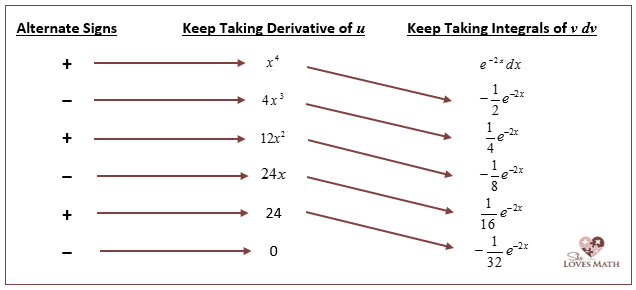
\includegraphics[height=.45\textheight]{line-method.png}\\
	\hspace*{10pt}\hbox{\thinspace{\tiny\itshape She Loves Math}}
\end{figure}

\end{frame}

\begin{frame}
\frametitle{Integration by Parts the Easy Way: Examples}
Integrate the following:
\begin{itemize}
	\item[(a)] $\int xe^{2x} \mathop{dx}$
	\item[(b)] $ \int_0^1 x^3 e^{2x} \mathop{dx}$
	\item[(c)] $\int_0^\pi x^2 \cos(4x) \mathop{dx}$
	\item[(d)]  $\int x^2 \ln 4x \mathop{dx} $
	\item[(e)] $\int \ln x \mathop{dx}$
	\item[(f)] $\int e^x \cos(x) \mathop{dx}$
\end{itemize}
\end{frame}

\begin{frame}
\frametitle{Improper Integrals}
An integral over an open interval or half open interval (eg: $(a,b]$) is called an improper integral. There are two types of improper integral. For instance consider
$$\int_{\infty}^{\infty} e^{-x^2} \mathop{dx} \mbox{ or } \int_0^5 \frac{1}{x^2} \mathop{dx}$$
Type I: One or both of the endpoints are infinite\\
Type II: The interval contains a point of discontinuity\\

\vspace{6pt}
An integral is \textit{divergent} if the evaluated integral is not a finite number or does not exist and \textit{convergent} if the evaluated integral is a finite number.
\end{frame}

\begin{frame}
\frametitle{Type I Improper Integrals}
\begin{itemize}
	\item[(i)] If $\int_{a}^{t} f(x) \mathop{dx}$ exists $\forall t \geq a$ then
	$$\int_{a}^{\infty}f(x) \mathop{dx} = \lim\limits_{t \to \infty} \int_a^tf(x) \mathop{dx}$$
	\item[(ii)] If $\int_{t}^{b} f(x) \mathop{dx}$ exists $\forall t \leq b$ then
	$$\int_{-\infty}^{b}f(x) \mathop{dx} = \lim\limits_{t \to -\infty} \int_t^bf(x) \mathop{dx}$$
	\item[(iii)] If  $\int_{a}^{t} f(x) \mathop{dx}$ and $\int_{t}^{a} f(x) \mathop{dx}$ exist $\forall a \in \mathbb{R}$ then
	$$\int_{-\infty}^\infty f(x) \mathop{dx} = \int_{-\infty}^a f(x) \mathop{dx} + \int_{a}^\infty f(x) \mathop{dx}$$
\end{itemize}

\vspace{6pt}
\textbf{Examples:}
\begin{itemize}
	\item[(a)] $\int_{1}^{\infty}\frac{1}{x} \mathop{dx}$
	\item[(b)] For what values of $p$ is $\int_{1}^{\infty}\frac{1}{x^p} \mathop{dx}$ convergent? (Assume $p \neq 1$.)
\end{itemize}
\end{frame}

\begin{frame}
\frametitle{Type II Improper Integrals}
\begin{itemize}
	\item[(i)]If $f$ is continuous on $[a,b)$ but discontinuous at $b$ then
	$$\int_a^bf(x) \mathop{dx} = \lim\limits_{t \to b^-} \int_{a}^{t}f(x)\mathop{dx}$$
	\item[(ii)]If $f$ is continuous on $(a,b]$ but discontinuous at $a$ then
	$$\int_a^bf(x) \mathop{dx} = \lim\limits_{t \to a^+} \int_{t}^{b}f(x)\mathop{dx}$$
	\item[(iii)] If $f$ has a discontinuity at $c \in [a,b]$ and both $\int_{a}^{c}f(x) \mathop{dx} \mbox{ and } \int_{c}^{b}f(x) \mathop{dx}$ converge then
	$$\int_a^bf(x) \mathop{dx} = \int_{a}^{c} f(x) \mathop{dx} + \int_{c}^{b} f(x) \mathop{dx}$$
\end{itemize}

\textbf{Examples:}
\begin{itemize}
	\item[(a)] $\int_{2}^{5}\frac{1}{\sqrt{x-2}} \mathop{dx}$
	\item[(b)] $\int_{-2}^{7}\frac{1}{(x+1)^{2/3}} \mathop{dx}$ 
\end{itemize}
\end{frame}

%\begin{frame}
%\frametitle{What is a Limit?}
%\begin{figure}
%	\centering
%	\begin{subfigure}{0.48\textwidth}
%		
%		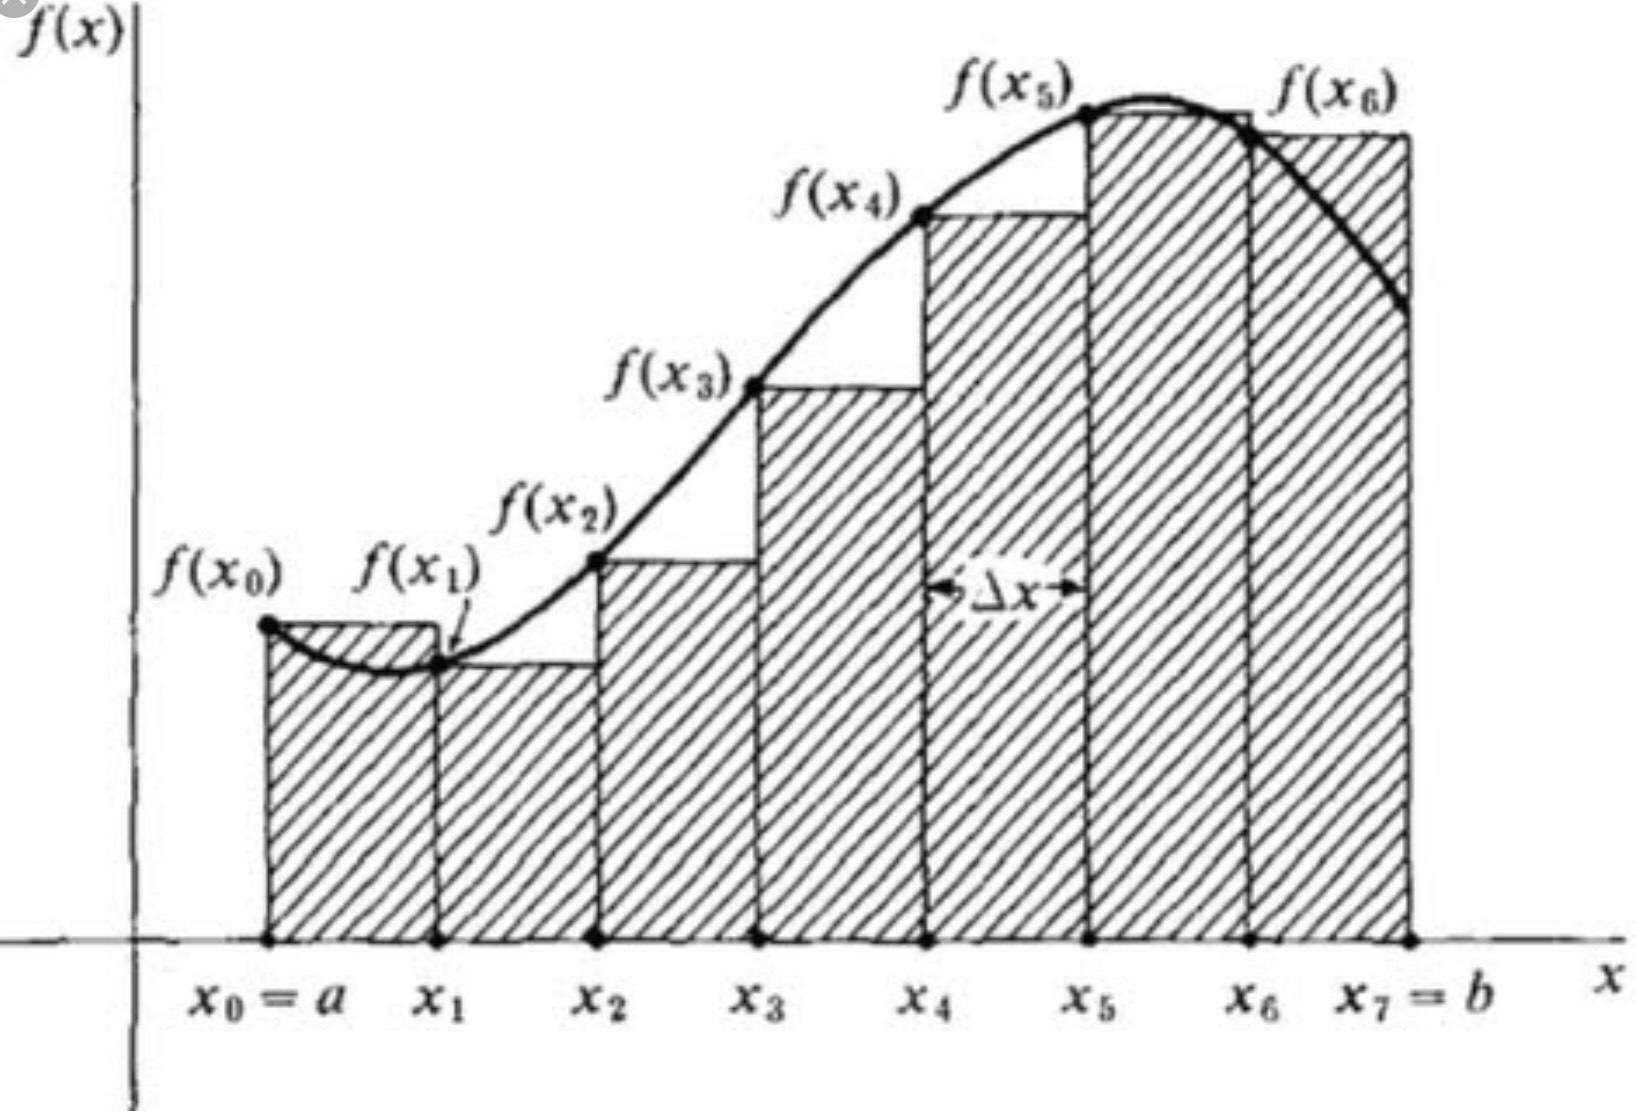
\includegraphics[width=\textwidth]{IMG_0380.jpg}
%		\hspace*{10pt}\hbox{\thinspace{\tiny\itshape vias.org}}
%		\caption{Single integration}
%	\end{subfigure}% 
%	~ 
%	\begin{subfigure}{0.48\textwidth}
%		
%		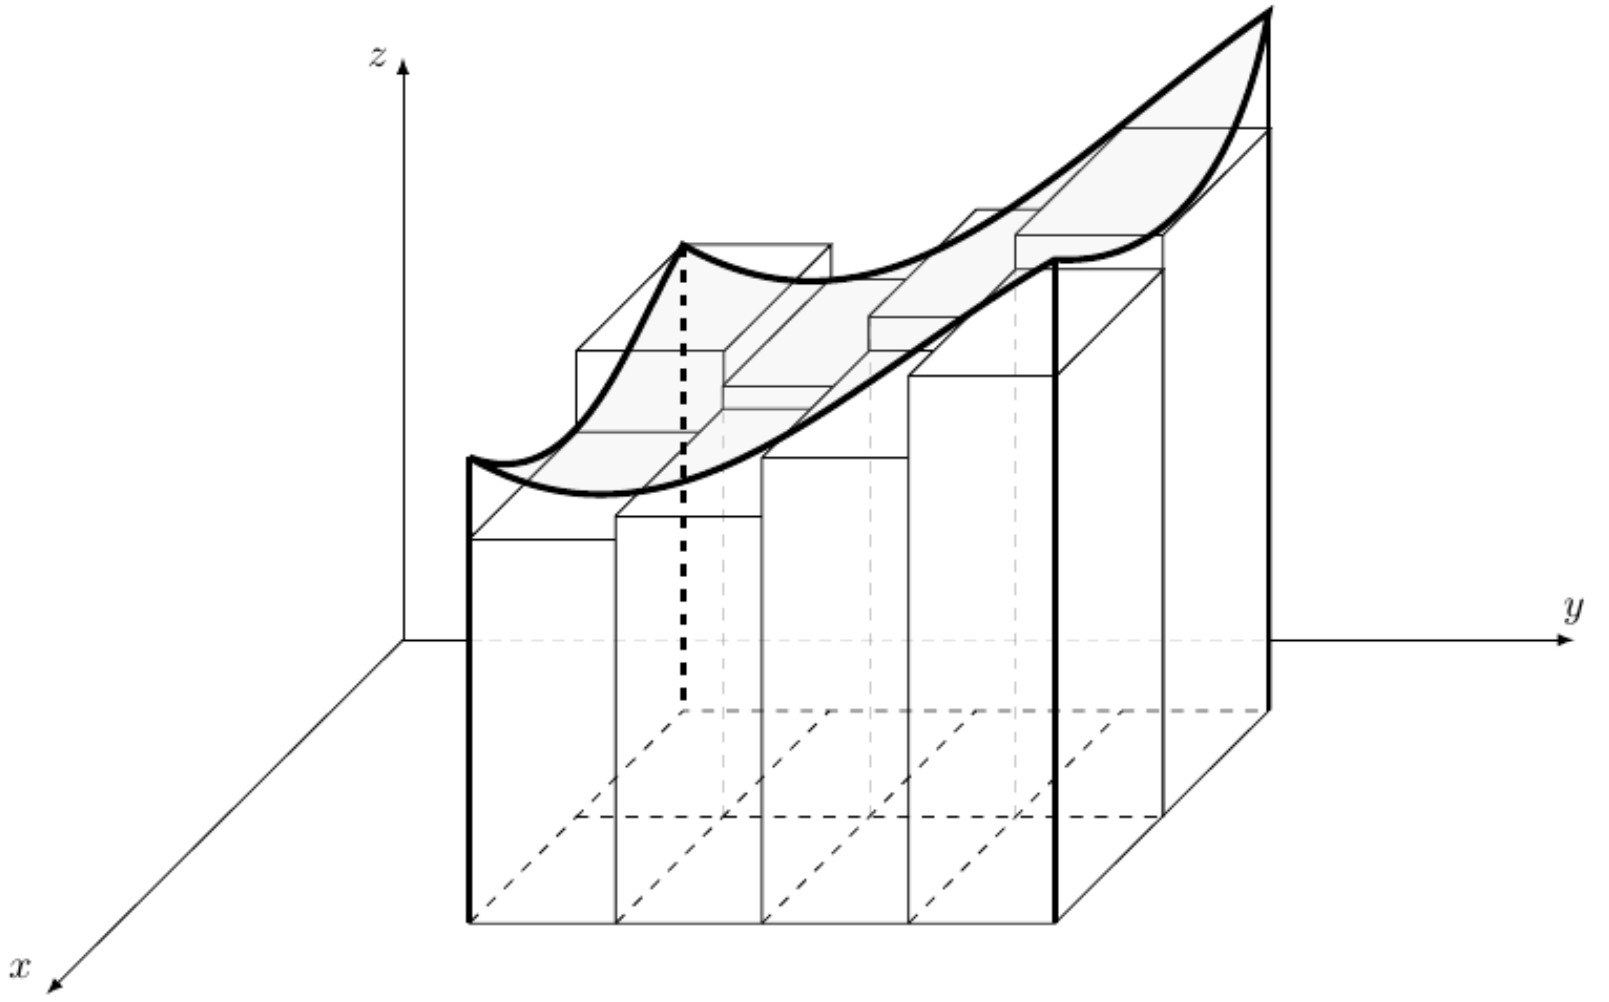
\includegraphics[width=\textwidth]{IMG_0385.jpg}
%		\hspace*{10pt}\hbox{\thinspace{\tiny\itshape tex.stackexchange.com}}
%		\caption{Double integration.}
%		\label{fig:2}
%	\end{subfigure}
%\end{figure}
%
%\end{frame}
%
%
%\begin{frame}
%\frametitle{Triple Integral}
%\begin{figure}
%	\centering
%	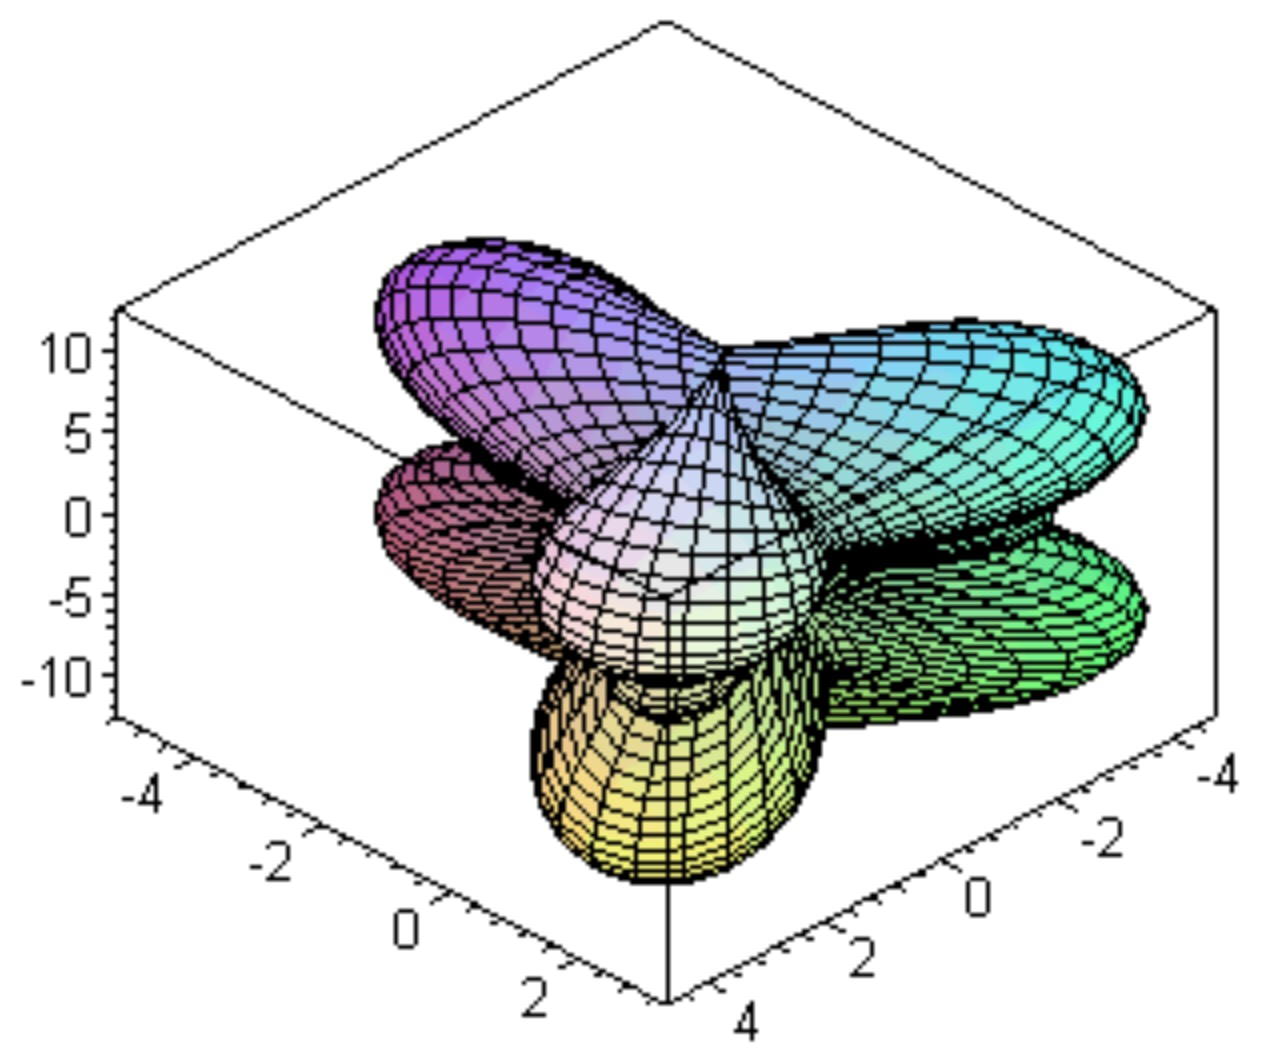
\includegraphics[height=.45\textheight]{IMG_0384.jpg}\\
%	\hspace*{10pt}\hbox{\thinspace{\tiny\itshape maplesoft.com}}
%\end{figure}
%
%$$\iiint\limits_{\mathbb{R}} F(x,y,z) dV = \int_{x=a}^{x=b} \int_{y=y_1(x)}^{y=y_2(x)} \int_{z=z_1(x,y)}^{z=z_2(x,y)} F(x,y,z) dz\,dy\,dx$$
%\textbf{Example:}
%\begin{itemize}
%	\item[(a)] $\int_0^1 \int_0^{1-x} \int_0^{2-x} xyz \,dz\,dy\,dx$
%\end{itemize}
%\end{frame}

\end{document}
